\def\title{Material de Apoyo}
\def\subtitle{Función afín}
\def\curso{Segundo medio}

\documentclass{caes}

\begin{document}

\titulo{Objetivos de la clase}
\begin{itemize}
    \item Ubicar puntos en el plano cartesiano.
    \item Identificar una función afín en alguna de sus tres representaciones distintas:
    tabla de puntos, gráfica en plano cartesiano o ecuación algebraica.
    \item A partir de una de las representaciones de la función afín, 
    encontrar las otras.
\end{itemize}

\titulo{Ticket de entrada}

\pregunta Considere la tabla de puntos y el plano cartesiano que se encuentra 
a continuación, mueva los puntos desde la tabla al plano cartesiano
y dibuje la recta que pasa por ellos. 

\def\tabla{%
\begin{mtabla}{}
    x & y \\
    0 & 0 \\
    1 & 2 \\
    4 & 8 \\
    5 & 10
\end{mtabla}
}
\def\grafica{%
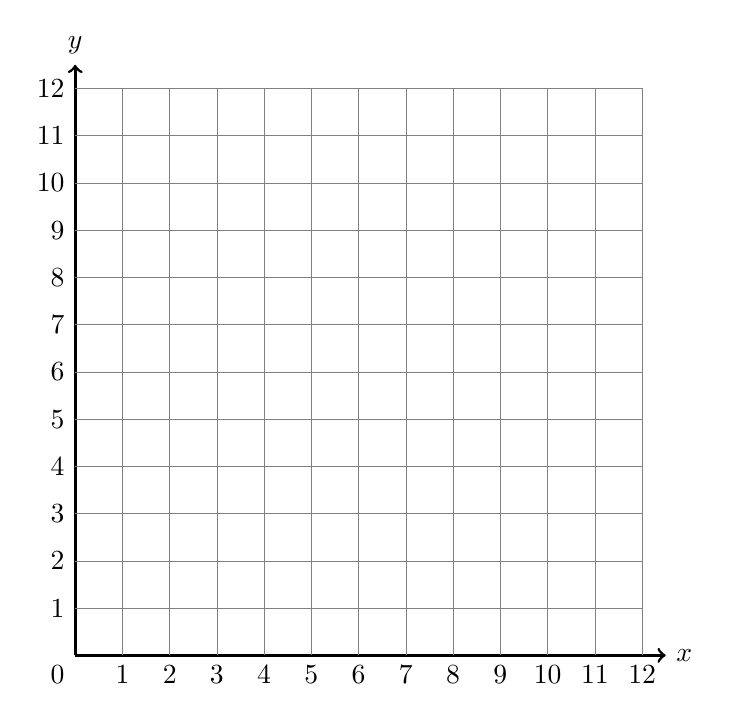
\begin{tikzpicture}[line width=1pt,x=0.6cm,y=0.6cm]
    \draw[->] (0,0) -- (12.5,0) node[right] {$x$};
    \foreach \x in {1,...,12} {
        \draw[help lines] (\x,0) -- (\x,12);
        \node[below] at (\x,0) {\x};
    }
    \draw[->] (0,0) -- (0,12.5) node[above] {$y$}; 
    \foreach \y in {1,...,12} {
        \draw[help lines] (0,\y) -- (12,\y);
        \node[left] at (0,\y) {\y};
    }
    \node[below left] at (0,0) {0};
\end{tikzpicture}
}

\begin{tikzpicture}
    \node (tabla) {\tabla};
    \node[left=2cm of tabla] (grafica) {\grafica}; 
\end{tikzpicture}

\pregunta Una vez dibujada la recta, encuentre la ecuación de dicha 
recta. 

\begin{center}
    \begin{tikzpicture}
        \node[text width=10cm,draw=primarycolor,dotted, line width=2pt, inner sep=5mm,rounded corners] {Recuerde que la ecuación de una recta es $y = m\cdot x + n$, 
        donde $m$ es la pendiente y $n$ el coeficiente de posición.};
    \end{tikzpicture}    
\end{center}
\desarrollo[3cm]

\newpage

\pregunta Repita los pasos anteriores para determinar la ecuación 
de la recta, usando la tabla y el plano cartesiano que se 
encuentran a continuación

\def\tabla{%
\begin{mtabla}{}
    x & y \\
    2 & 1 \\
    4 & 7 \\
    5 & 10
\end{mtabla}
}
\def\grafica{%
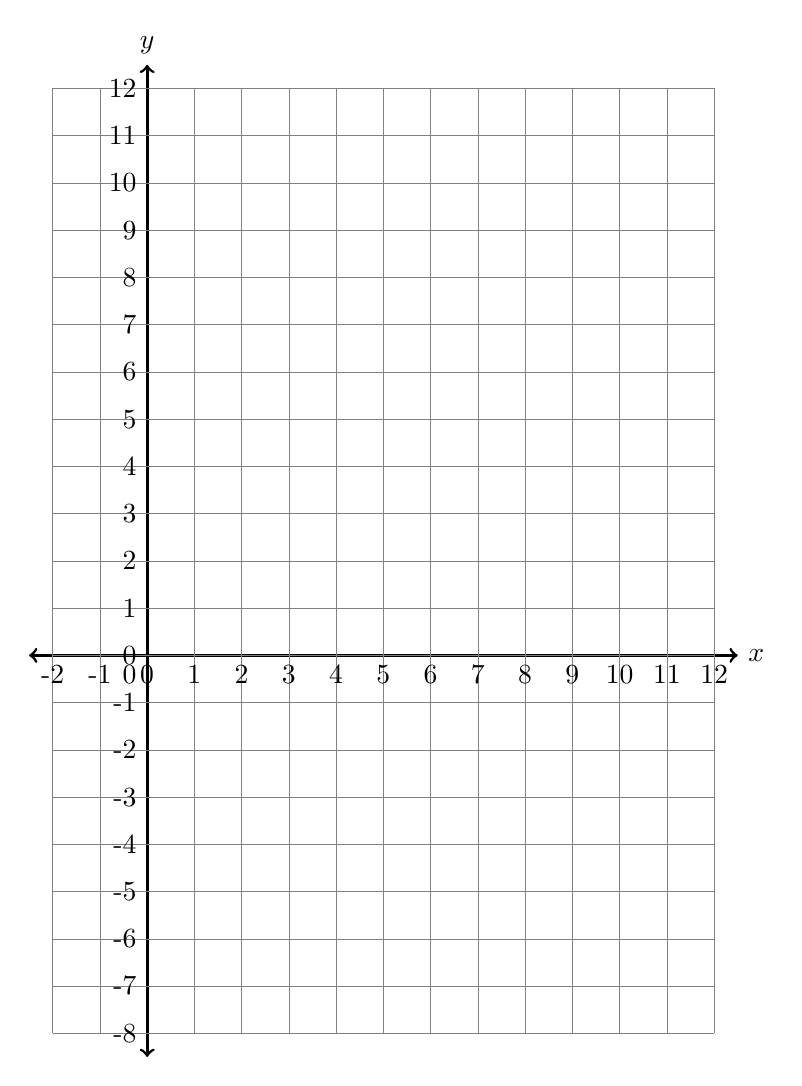
\begin{tikzpicture}[line width=1pt,x=0.6cm,y=0.6cm]
    \draw[<->] (-2.5,0) -- (12.5,0) node[right] {$x$};
    \foreach \x in {-2,...,12} {
        \draw[help lines] (\x,-8) -- (\x,12);
        \ifthenelse{\x=0}{}{\node[below] at (\x,0) {\x};}
    }
    \draw[<->] (0,-8.5) -- (0,12.5) node[above] {$y$}; 
    \foreach \y in {-8,...,12} {
        \draw[help lines] (-2,\y) -- (12,\y);
        \ifthenelse{\y=0}{}{\node[left] at (0,\y) {\y};}
    }
    \node[below left] at (0,0) {0};
\end{tikzpicture}
}
\begin{tikzpicture}
    \node (tabla) {\tabla};
    \node[left=2cm of tabla] (grafica) {\grafica}; 
\end{tikzpicture}
\desarrollo[3cm]

\newpage

\titulo{Procedimiento para encontrar la ecuación de una recta}
\begin{enumerate}
    \item Marcar los puntos en el plano cartesiano y trazar la 
    recta que pasa por ellos.
    \item Calcular la pendiente ($\boldsymbol m$) usando los triángulos que
    se forman entre la recta y el plano cartesiano. {\bfseries La 
    pendiente corresponde división entre el lado vertical y el
    horizontal del triángulo}.
    \item {\bfseries El coeficiente de posición ($\boldsymbol n$) corresponde a la posición
    por donde la recta atraviesa el eje $\boldsymbol y$.} En caso de 
    no conocer este punto de intersección, usar el valor de $m$ 
    encontrado anteriormente y un punto conocido de la función 
    para despejar $n$ en la ecuación $y = m\cdot x + n$.
    \item Finalmente, la ecuación de la recta es $y = m\cdot x + n$ con
    $m$ y $n$ conocidos.
\end{enumerate}

\titulo{Ticket de salida}

\pregunta Use el procedimiento visto en clases, para encontrar 
la ecuación de la recta correspondiente a la \\siguiente tabla

\def\tabla{%
\begin{mtabla}{}
    x & y\\
    -4 & 4 \\
    4  &-3 
\end{mtabla}
}
\def\grafica{%
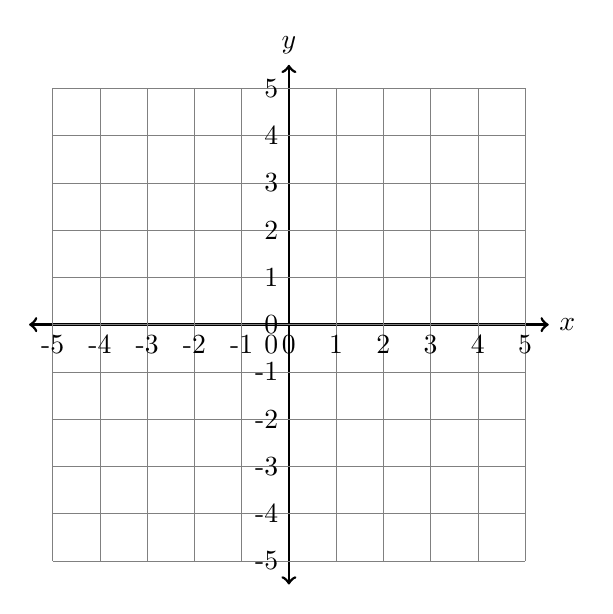
\begin{tikzpicture}[line width=1pt,x=0.6cm,y=0.6cm]
    \draw[<->] (-5.5,0) -- (5.5,0) node[right] {$x$};
    \foreach \x in {-5,...,5} {
        \draw[help lines] (\x,-5) -- (\x,5);
        \ifthenelse{\x=0}{}{\node[below] at (\x,0) {\x};}
    }
    \draw[<->] (0,-5.5) -- (0,5.5) node[above] {$y$}; 
    \foreach \y in {-5,...,5} {
        \draw[help lines] (-5,\y) -- (5,\y);
        \ifthenelse{\y=0}{}{\node[left] at (0,\y) {\y};}
    }
    \node[below left] at (0,0) {0};
\end{tikzpicture}
}

\begin{tikzpicture}
    \node (tabla) {\tabla};
    \node[left=2cm of tabla] (grafica) {\grafica}; 
\end{tikzpicture}

\desarrollo[5cm]


\end{document}